\documentclass[dvipdfmx,a4j]{jarticle}
\setlength{\textheight}{23.5cm}
\usepackage{tikz}
\usetikzlibrary{automata,calc,shapes,math}
\pagestyle{empty}
\newcounter{coffee}
\newcounter{bean}
\newcommand{\ttpl}{\texttt{+}}
\newcommand{\ttmu}{\texttt{*}}
\newcommand{\tta}{\texttt{a}}
\newcommand{\ttx}{\texttt{x}}
\newcommand{\tteq}{\texttt{=}}
\newcommand{\ttlt}{\texttt{<}}
\newcommand{\ttsb}{\texttt{-}}
\newcommand{\eof}{\texttt{\#}}
\newcommand{\actrec}[3]{
  \coordinate (framebase) at #1;
  \draw (framebase) rectangle +(2,1);
  \node at ($(framebase)+(0.5,+0.25)$) {rv};
  \node at ($(framebase)+(0.5,+0.75)$) {\ttx};
  \node at ($(framebase)+(1.5,+0.25)$) {#2};
  \node at ($(framebase)+(1.5,+0.75)$) {#3};  
}
\newcommand{\actbase}[1]{
  \coordinate (actbase) at #1;
  \node at ($(actbase)+(0.5,-0.25)$) {\tta};
  \node at ($(actbase)+(1.5,-0.25)$) {3};
  \draw (actbase) rectangle +(2,-0.5);
}
\newcommand{\temprv}[2]{
  \coordinate (tempbase) at #1;
  \draw #1 rectangle +(2,0.5);
  \draw ($#1+(1,0)$) + (0,0.5);
  \node at ($#1+(0.5,0.25)$) {};
  \node at ($#1+(1.5,0.25)$) {#2};
}
\newcommand{\calltrans}[2]{
  \coordinate (callbase) at #1;
  \path[->] ($(callbase)+(0.25,0)$) edge [above] node {#2} +(1.5,0);
}
\newcommand{\tmpv}[1]{\texttt{t}_{#1}}
\begin{document}
% \begin{flushright}
% \end{flushright}
\begin{center}
    {\bf\Large コンパイラ演習課題(5)(解答例)}
\end{center}

\begin{list}{[\arabic{coffee}]}{\usecounter{coffee}}
  \item \ \\
  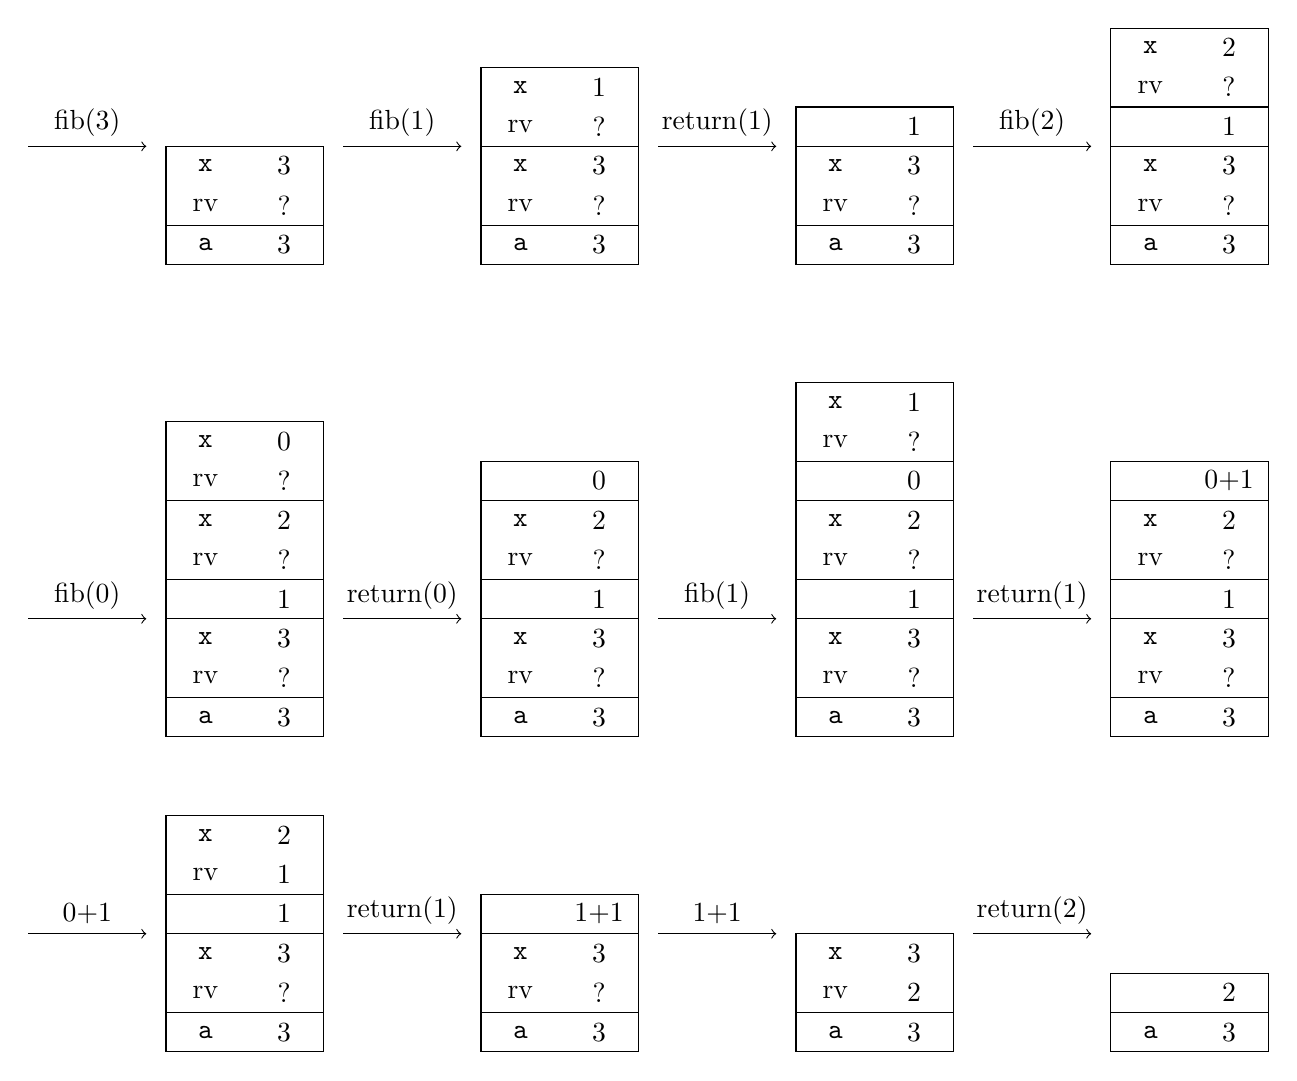
\begin{tikzpicture}
  \coordinate (fib3) at (0,0);
  \calltrans{(fib3)}{fib(3)}
  \actbase{($(fib3)+(2,-1)$)}
  \actrec{($(fib3)+(2,-1)$)}{?}{3}
  %
  \coordinate (fib1) at (4,0);
  \calltrans{(fib1)}{fib(1)}
  \actbase{($(fib1)+(2,-1)$)}
  \actrec{($(fib1)+(2,-1)$)}{?}{3}
  \actrec{($(fib1)+(2,0)$)}{?}{1}
  %
  \coordinate (ret1) at (8,0);
  \calltrans{(ret1)}{return(1)}
  \actbase{($(ret1)+(2,-1)$)}
  \actrec{($(ret1)+(2,-1)$)}{?}{3}
  \temprv{($(ret1)+(2,0)$)}{1}
  %
  \coordinate (fib2) at (12,0);
  \calltrans{(fib2)}{fib(2)}
  \actbase{($(fib2)+(2,-1)$)}
  \actrec{($(fib2)+(2,-1)$)}{?}{3}
  \temprv{($(fib2)+(2,0)$)}{1}
  \actrec{($(fib2)+(2,0.5)$)}{?}{2}
  %
  \coordinate (fib0) at (0,-6);
  \calltrans{(fib0)}{fib(0)}
  \actbase{($(fib0)+(2,-1)$)}
  \actrec{($(fib0)+(2,-1)$)}{?}{3}
  \temprv{($(fib0)+(2,0)$)}{1}
  \actrec{($(fib0)+(2,0.5)$)}{?}{2}
  \actrec{($(fib0)+(2,1.5)$)}{?}{0}
  %
  \coordinate (return0) at (4,-6);
  \calltrans{(return0)}{return(0)}
  \actbase{($(return0)+(2,-1)$)}
  \actrec{($(return0)+(2,-1)$)}{?}{3}
  \temprv{($(return0)+(2,0)$)}{1}
  \actrec{($(return0)+(2,0.5)$)}{?}{2}
  \temprv{($(return0)+(2,1.5)$)}{0}
  %
  \coordinate (fib1@1) at (8,-6);
  \calltrans{(fib1@1)}{fib(1)}
  \actbase{($(fib1@1)+(2,-1)$)}
  \actrec{($(fib1@1)+(2,-1)$)}{?}{3}
  \temprv{($(fib1@1)+(2,0)$)}{1}
  \actrec{($(fib1@1)+(2,0.5)$)}{?}{2}
  \temprv{($(fib1@1)+(2,1.5)$)}{0}
  \actrec{($(fib1@1)+(2,2)$)}{?}{1}
  %
  \coordinate (ret1@1) at (12,-6);
  \calltrans{(ret1@1)}{return(1)}
  \actbase{($(ret1@1)+(2,-1)$)}
  \actrec{($(ret1@1)+(2,-1)$)}{?}{3}
  \temprv{($(ret1@1)+(2,0)$)}{1}
  \actrec{($(ret1@1)+(2,0.5)$)}{?}{2}
  \temprv{($(ret1@1)+(2,1.5)$)}{0+1}
  %
  \coordinate (0plus1) at (0,-10);
  \calltrans{(0plus1)}{0+1}
  \actbase{($(0plus1)+(2,-1)$)}
  \actrec{($(0plus1)+(2,-1)$)}{?}{3}
  \temprv{($(0plus1)+(2,0)$)}{1}
  \actrec{($(0plus1)+(2,0.5)$)}{1}{2}
  %
  \coordinate (ret1@2) at (4,-10);
  \calltrans{(ret1@2)}{return(1)}  
  \actbase{($(ret1@2)+(2,-1)$)}
  \actrec{($(ret1@2)+(2,-1)$)}{?}{3}
  \temprv{($(ret1@2)+(2,0)$)}{1+1}
  %
  \coordinate (1plus1) at (8,-10);
  \calltrans{(1plus1)}{1+1}  
  \actbase{($(1plus1)+(2,-1)$)}
  \actrec{($(1plus1)+(2,-1)$)}{2}{3}
  %
  \coordinate (ret2) at (12,-10);
  \calltrans{(ret2)}{return(2)}  
  \actbase{($(ret2)+(2,-1)$)}
  \temprv{($(ret2)+(2,-1)$)}{2}
  \end{tikzpicture}
  
\item 
\begin{list}{(\alph{bean})}{\usecounter{bean}}
\item (1) $\{S.label1:=\mathsf{\mathsf{newLabel}}(); \mathsf{generate}(S.label1)\}$\\
(2) $\{\mathsf{generate}(\texttt{if}\ E.var\ \texttt{goto}\ S.label1)\}$
\item \[\begin{array}{lll}
  {\tt label}\ \ell_0: & // & S.label:=\mathsf{newLabel}(); \mathsf{generate}({\tt label}\ S.label1);\\
\tmpv{1} \tteq x1 & // & \tmpv{1}{\rm :=}\mathsf{newTemp}()\ \mbox{for $C.var$}\\
\tmpv{2} \tteq \tmpv{1} & // &  \tmpv{2}{\rm :=}\mathsf{newTemp}()\ \mbox{for $D.var$}\\
\tmpv{3} \tteq x2 & // & \tmpv{3}{\rm :=}\mathsf{newTemp}()\ \mbox{for $C.var$}\\
\tmpv{4} \tteq \tmpv{2}\ttlt\tmpv{3} & // & \tmpv{4}{\rm :=}\mathsf{newTemp}()\ \mbox{for $D.var$}\\
\tmpv{5} \tteq \tmpv{4} & // & \tmpv{5}{\rm :=}\mathsf{newTemp}()\ \mbox{for $E.var$}\\
{\tt if\_not}\ \tmpv{5}\ \texttt{goto}\ \ell_1;\\
\tmpv{6} \tteq x1 & // & \tmpv{6}{\rm :=}\mathsf{newTemp}()\ \mbox{for $C.var$}\\
\tmpv{7} \tteq \tmpv{6}\ttsb x3 & // & \tmpv{7}{\rm :=}\mathsf{newTemp}()\ \mbox{for $C.var$}\\
\tmpv{8} \tteq \tmpv{7} & // & \tmpv{8}{\rm :=}\mathsf{newTemp}()\ \mbox{for $D.var$}\\
\tmpv{9} \tteq \tmpv{8} & // & \tmpv{8}{\rm :=}\mathsf{newTemp}()\ \mbox{for $E.var$}\\
x1 \tteq \tmpv{9}\\
{\tt goto}\ \ell_2\\
{\tt label}\ \ell_1: & // & S^{(1)}.label1:=\mathsf{newLabel}(); \mathsf{generate}({\tt label}\ S^{(1)}.label1);\\
\tmpv{10} \tteq x2 & // & \tmpv{10}{\rm :=}\mathsf{newTemp}()\ \mbox{for $C.var$}\\
\tmpv{11} \tteq \tmpv{10}\ttsb x4 & // & \tmpv{11}{\rm :=}\mathsf{newTemp}()\ \mbox{for $C.var$}\\
\tmpv{12} \tteq \tmpv{11} & // & \tmpv{12}{\rm :=}\mathsf{newTemp}()\ \mbox{for $D.var$}\\
\tmpv{13} \tteq \tmpv{12} & // & \tmpv{13}{\rm :=}\mathsf{newTemp}()\ \mbox{for $E.var$}\\
x2 \tteq \tmpv{13}\\
{\tt label}\ \ell_2 : & // & S^{(1)}.label2:=\mathsf{newLabel}(); \mathsf{generate}({\tt label}\ S^{(1)}.label2);\\
\tmpv{14} \tteq x5 & // & \tmpv{14}{\rm :=}\mathsf{newTemp}()\ \mbox{for $C.var$}\\
\tmpv{15} \tteq \tmpv{14} & // & \tmpv{15}{\rm :=}\mathsf{newTemp}()\ \mbox{for $D.var$}\\
\tmpv{16} \tteq x1 & // & \tmpv{16}{\rm :=}\mathsf{newTemp}()\ \mbox{for $C.var$}\\
\tmpv{17} \tteq \tmpv{16}\ttsb x6 & // & \tmpv{17}{\rm :=}\mathsf{newTemp}()\ \mbox{for $C.var$}\\
\tmpv{18} \tteq \tmpv{14}\ttlt\tmpv{17} & // & \tmpv{18}{\rm :=}\mathsf{newTemp}()\ \mbox{for $D.var$}\\
\tmpv{19} \tteq \tmpv{18} & // & \tmpv{19}{\rm :=}\mathsf{newTemp}()\ \mbox{for $E.var$}\\
\tmpv{20} \tteq x7 & // & \tmpv{20}{\rm :=}\mathsf{newTemp}()\ \mbox{for $C.var$}\\
\tmpv{21} \tteq \tmpv{20} & // & \tmpv{21}{\rm :=}\mathsf{newTemp}()\ \mbox{for $D.var$}\\
\tmpv{22} \tteq x1 & // & \tmpv{22}{\rm :=}\mathsf{newTemp}()\ \mbox{for $C.var$}\\
\tmpv{23} \tteq \tmpv{21}\ttlt\tmpv{22} & // & \tmpv{23}{\rm :=}\mathsf{newTemp}()\ \mbox{for $D.var$}\\
\tmpv{24} \tteq \tmpv{19}\ \texttt{AND}\ \tmpv{23} & // & \tmpv{24}{\rm :=}\mathsf{newTemp}()\ \mbox{for $E.var$}\\
{\tt if}\ \tmpv{24}\ {\tt goto}\ \ell_0\\
  \end{array}\]
\end{list}

\end{list}
\end{document}